% ============================================================
% 第四章 动力系统设计与选型
% ============================================================

\chapter{动力系统设计与选型}

\section{整机质量预算}

动力系统选型的首要输入参数是整机起飞质量。
本系统对各部件质量进行系统梳理与预算，
所有数值以实物称重或厂商规格表数据为准，如表~\ref{tab:mass_budget}所示。

\begin{longtable}{llr}
    \caption{整机质量预算}
    \label{tab:mass_budget} \\

    % -------- 第一页表头 --------
    \toprule
    部件 & 型号/说明 & 质量 (g) \\
    \midrule
    \endfirsthead

    % -------- 续页表头 --------
    \multicolumn{3}{l}{\small 续表~\ref*{tab:mass_budget}} \\[2pt]
    \toprule
    部件 & 型号/说明 & 质量 (g) \\
    \midrule
    \endhead

    % -------- 每页底部（非末页）--------
    \midrule
    \multicolumn{3}{r}{\small 接下页} \\
    \endfoot

    % -------- 最后一页底部 --------
    \bottomrule
    \endlastfoot

    % -------- 表格内容 --------
    无刷电机 $\times 4$          & SIRIUS 2306.5-1850KV & 320 \\[3pt]
    电子调速器（ESC）$\times 4$  & —                    & 100 \\[3pt]
    桨叶 $\times 4$              & 51366 MCK v3         &  52 \\[3pt]
    飞行控制器                   & Pixhawk 6C           &  38 \\[3pt]
    GPS模块                      & —                    &  30 \\[3pt]
    遥控接收机                   & 乐迪 R9DS            &  15 \\[3pt]
    PLA节点结构件                & FDM 3D打印           & 600 \\[3pt]
    气柱骨架（全部）             & 快递气柱             & 150 \\[3pt]
    TPU伞面                      & TPU薄膜              & 150 \\[3pt]
    线缆与紧固件                 & —                    &  13 \\
    \midrule
    \textbf{整机合计}            & —                    & \textbf{1468} \\

\end{longtable}
电源延长线（14AWG，约150cm）对系统重心影响极小可忽略。
因此，整机起飞质量 $m = 1468$\,g（不含地面系留电源），
对应总重力：

\begin{equation}
    W = mg = 1.468 \times 9.81 = 14.40\,\text{N}
    \label{eq:weight}
\end{equation}

系统在悬停状态下所需的四旋翼总升力须满足 $T_{\text{total}} \geq W = 14.40$\,N。


\section{悬停升力需求与动量理论分析}

\subsection{悬停升力需求}

在静态悬停条件下，飞行器所需总升力等于整机重力，即：

\begin{equation}
    T_{\text{total}} = W = 14.40\,\text{N}
    \label{eq:hover_thrust}
\end{equation}

四旋翼对称布局下，单旋翼所需悬停升力为：

\begin{equation}
    T_{\text{single}} = \frac{T_{\text{total}}}{4} = \frac{14.40}{4} = 3.60\,\text{N} \approx 367\,\text{gf}
    \label{eq:single_thrust}
\end{equation}

\subsection{动量理论推导}

根据螺旋桨动量理论（Actuator Disk Theory），
旋翼在悬停状态下通过加速桨盘下方气流产生升力。
设桨盘面积为 $A$，气流诱导速度为 $v_i$，在无损理想情况下，推力与诱导速度的关系为：

\begin{equation}
    T = 2\rho A v_i^2
    \label{eq:momentum_theory}
\end{equation}

由此可解出悬停诱导速度：

\begin{equation}
    v_i = \sqrt{\frac{T}{2\rho A}}
    \label{eq:induced_velocity}
\end{equation}

本系统选用51366 MCK v3桨叶，桨盘直径 $D = 5.1$\,inch $= 129.5$\,mm，
对应桨盘面积：

\begin{equation}
    A = \pi \left(\frac{D}{2}\right)^2 = \pi \times (0.0648)^2 \approx 1.318 \times 10^{-2}\,\text{m}^2
    \label{eq:disk_area}
\end{equation}

取标准大气密度 $\rho = 1.225$\,kg/m$^3$，代入式~(\ref{eq:induced_velocity})：

\begin{equation}
    v_i = \sqrt{\frac{3.60}{2 \times 1.225 \times 1.318 \times 10^{-2}}} \approx 10.56\,\text{m/s}
    \label{eq:vi_result}
\end{equation}

\subsection{悬停功率估算}
根据动量理论，单旋翼的理想悬停诱导功率 $P_{i,\text{single}}$ 为推力与诱导速度的乘积：
\begin{equation}
    P_{i,\text{single}} = T_{\text{single}} v_i = 3.60 \times 10.56 \approx 38.02\,\text{W}
    \label{eq:ideal_power_single}
\end{equation}
四旋翼系统的总理想悬停功率为 $P_{i,\text{total}} = 4 \times 38.02 \approx 152.1\,\text{W}$。

在实际运行中，考虑到桨叶的叶型阻力、桨尖损失以及电机的机电转换损耗，
引入悬停效率系数（Figure of Merit, FM）进行修正。
结合所选电机与桨叶的测试经验数据，取综合效率系数 $\text{FM} = 0.70$，
则系统实际悬停总功率估算为：
\begin{equation}
    P_{\text{actual}} = \frac{P_{i,\text{total}}}{\text{FM}} = \frac{152.1}{0.70} \approx 217\,\text{W}
    \label{eq:actual_power}
\end{equation}
此功率值将作为后续续航时间估算的基准输入。


\section{电机与桨叶选型}

\subsection{选型依据}

基于上节计算，单旋翼悬停推力需求为367\,gf，
系统对电机选型提出以下约束条件：

\begin{itemize}
    \item 推力：在合理油门（$\leq 70\%$）下单电机推力须 $\geq 550$\,gf，
          以保证推重比 $\geq 1.5$；
    \item 效率：悬停工作点效率（g/W）尽量高，以延长续航时间；
    \item 重量：单电机质量 $\leq 100$\,g（四电机合计 $\leq 400$\,g）；
    \item 适配性：电机安装孔径与旋翼保护圈结构兼容。
\end{itemize}

\subsection{电机选型：SIRIUS 2306.5-1850KV}

本系统选用 \textbf{SIRIUS 2306.5-1850KV} 无刷电机，主要参数如表~\ref{tab:motor_spec}所示。

\begin{longtable}{ll}
    \caption{SIRIUS 2306.5-1850KV 电机主要参数}
    \label{tab:motor_spec} \\

    % -------- 第一页表头 --------
    \toprule
    参数 & 数值 \\
    \midrule
    \endfirsthead

    % -------- 续页表头 --------
    \multicolumn{2}{l}{\small 续表~\ref*{tab:motor_spec}} \\[2pt]
    \toprule
    参数 & 数值 \\
    \midrule
    \endhead

    % -------- 每页底部（非末页）--------
    \midrule
    \multicolumn{2}{r}{\small 接下页} \\
    \endfoot

    % -------- 最后一页底部 --------
    \bottomrule
    \endlastfoot

    % -------- 表格内容 --------
    定子尺寸     & 23\,mm $\times$ 6.5\,mm \\[3pt]
    KV值        & 1850\,rpm/V \\[3pt]
    推荐电池     & 4S $\sim$ 6S \\[3pt]
    单机质量     & 约 80\,g \\[3pt]
    最大连续电流  & 约 35\,A \\

\end{longtable}

% 电机图：左侧实物图 + 右侧工程图
SIRIUS~2306.5-1850KV 电机外观与尺寸如图~\ref{fig:motor}所示。

\begin{figure}[htbp]
    \centering
    \begin{subfigure}[b]{0.45\textwidth}
        \centering
        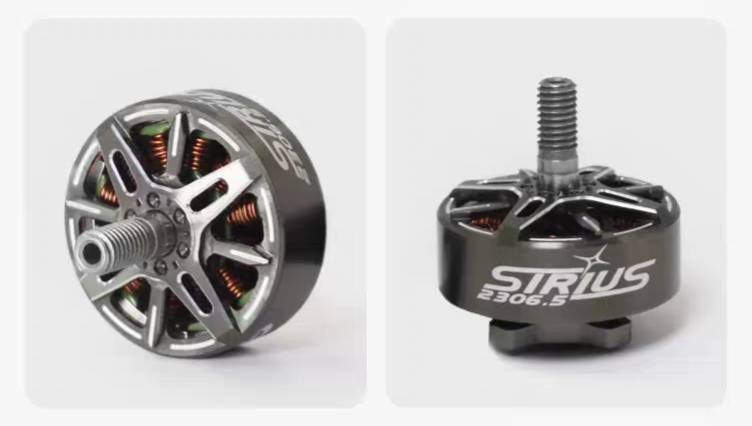
\includegraphics[width=\textwidth]{figures/fig4_2_motor_photo.jpeg}
        \caption{实物图}
        \label{fig:motor_photo}
    \end{subfigure}
    \hfill
    \begin{subfigure}[b]{0.45\textwidth}
        \centering
        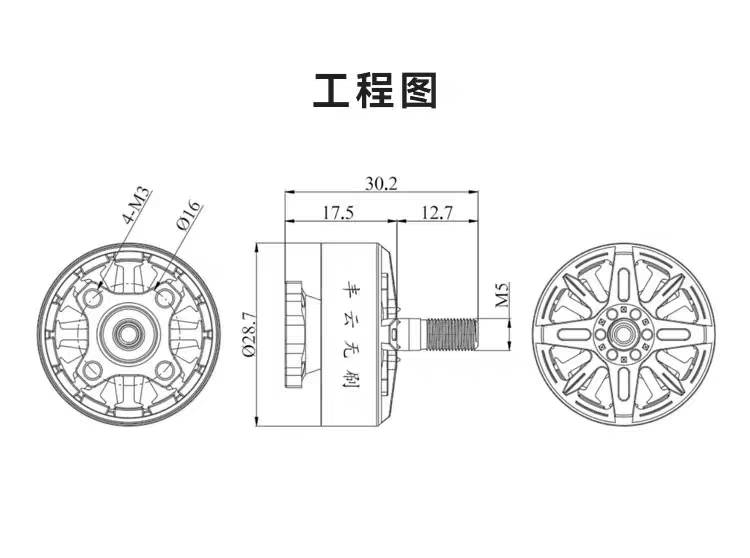
\includegraphics[width=\textwidth]{figures/fig4_2_motor_drawing.jpeg}
        \caption{工程图}
        \label{fig:motor_drawing}
    \end{subfigure}
    \caption{SIRIUS 2306.5-1850KV 无刷电机}
    \label{fig:motor}
\end{figure}

\subsection{桨叶选型：51366 MCK v3}
配套选用 \textbf{51366 MCK v3} 桨叶，直径5.1\,inch。
该桨叶实物如图~\ref{fig:propeller}所示。

\begin{figure}[htbp]
    \centering
    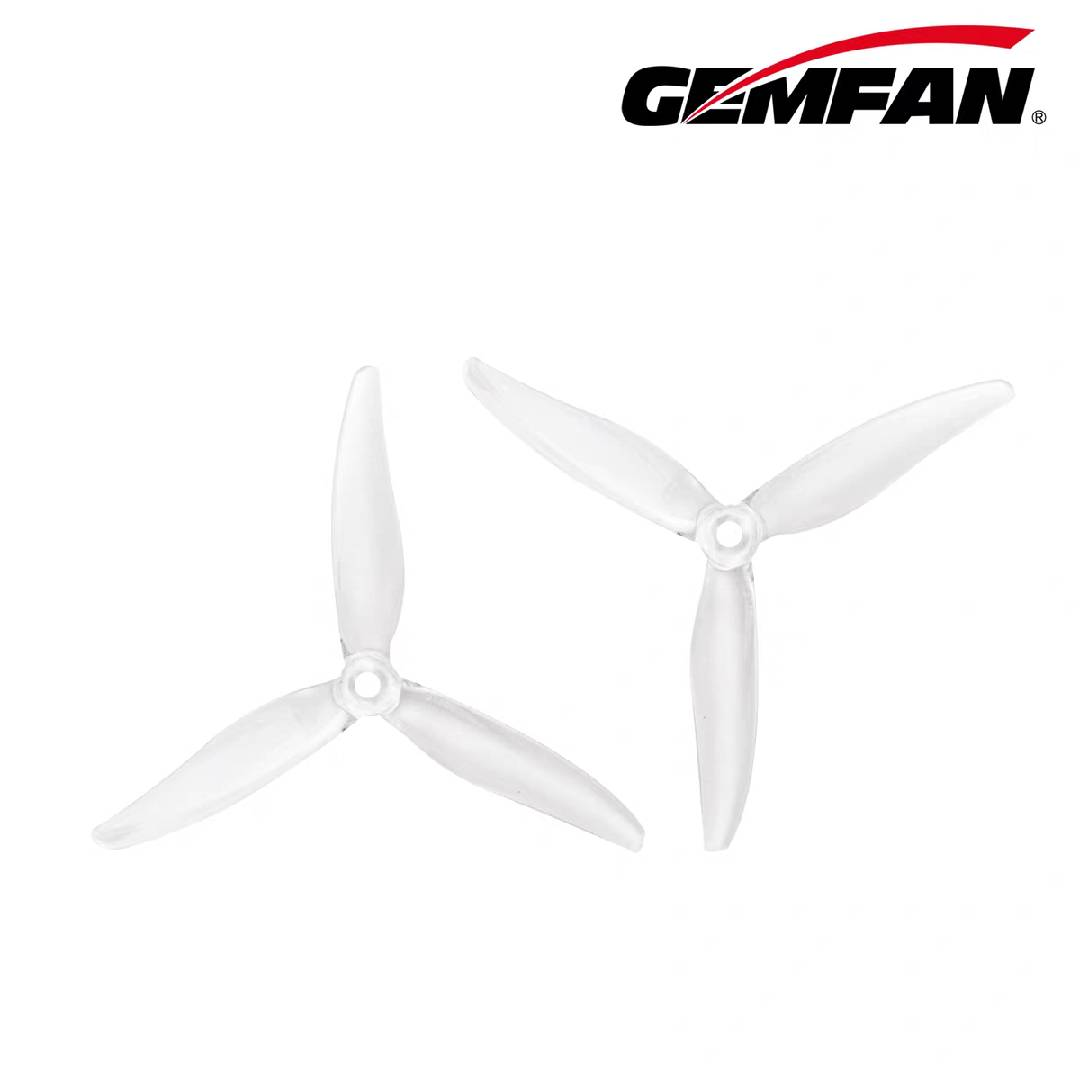
\includegraphics[width=0.30\textwidth]{figures/fig4_3_propeller_photo.jpeg}
    \caption{51366 MCK v3 桨叶实物图}
    \label{fig:propeller}
\end{figure}

在 6S（22.2\,V）电压下，配合 2100KV 级别电机使用时，
官方静态测试的典型推力-油门数据如表~\ref{tab:thrust_data}所示。

\begin{longtable}{lrrr}
    \caption{51366 MCK v3 桨叶推力测试数据（6S，四旋翼合计）}
    \label{tab:thrust_data} \\
    % -------- 第一页表头 --------
    \toprule
    油门（\%） & 单旋翼推力 (gf) & 四旋翼合计 (gf) & 推重比 \\
    \midrule
    \endfirsthead
    % -------- 续页表头 --------
    \multicolumn{4}{l}{\small 续表~\ref*{tab:thrust_data}} \\[2pt]
    \toprule
    油门（\%） & 单旋翼推力 (gf) & 四旋翼合计 (gf) & 推重比 \\
    \midrule
    \endhead
    % -------- 每页底部（非末页）--------
    \midrule
    \multicolumn{4}{r}{\small 接下页} \\
    \endfoot
    % -------- 最后一页底部 --------
    \bottomrule
    \endlastfoot
    % -------- 表格内容 --------
    30\%  &  205  &  820  & 0.56 \\[3pt]
    40\%  &  399  & 1596  & 1.09 \\[3pt]
    50\%  &  591  & 2364  & 1.61 \\[3pt]
    70\%  & 1113  & 4452  & 3.03 \\[3pt]
    90\%  & 1576  & 6304  & 4.29 \\
\end{longtable}


为了更直观地展示系统的动力冗余情况，绘制了如图~\ref{fig:thrust_curve}所示的推力-油门关系曲线。

\begin{figure}[htbp]
    \centering
    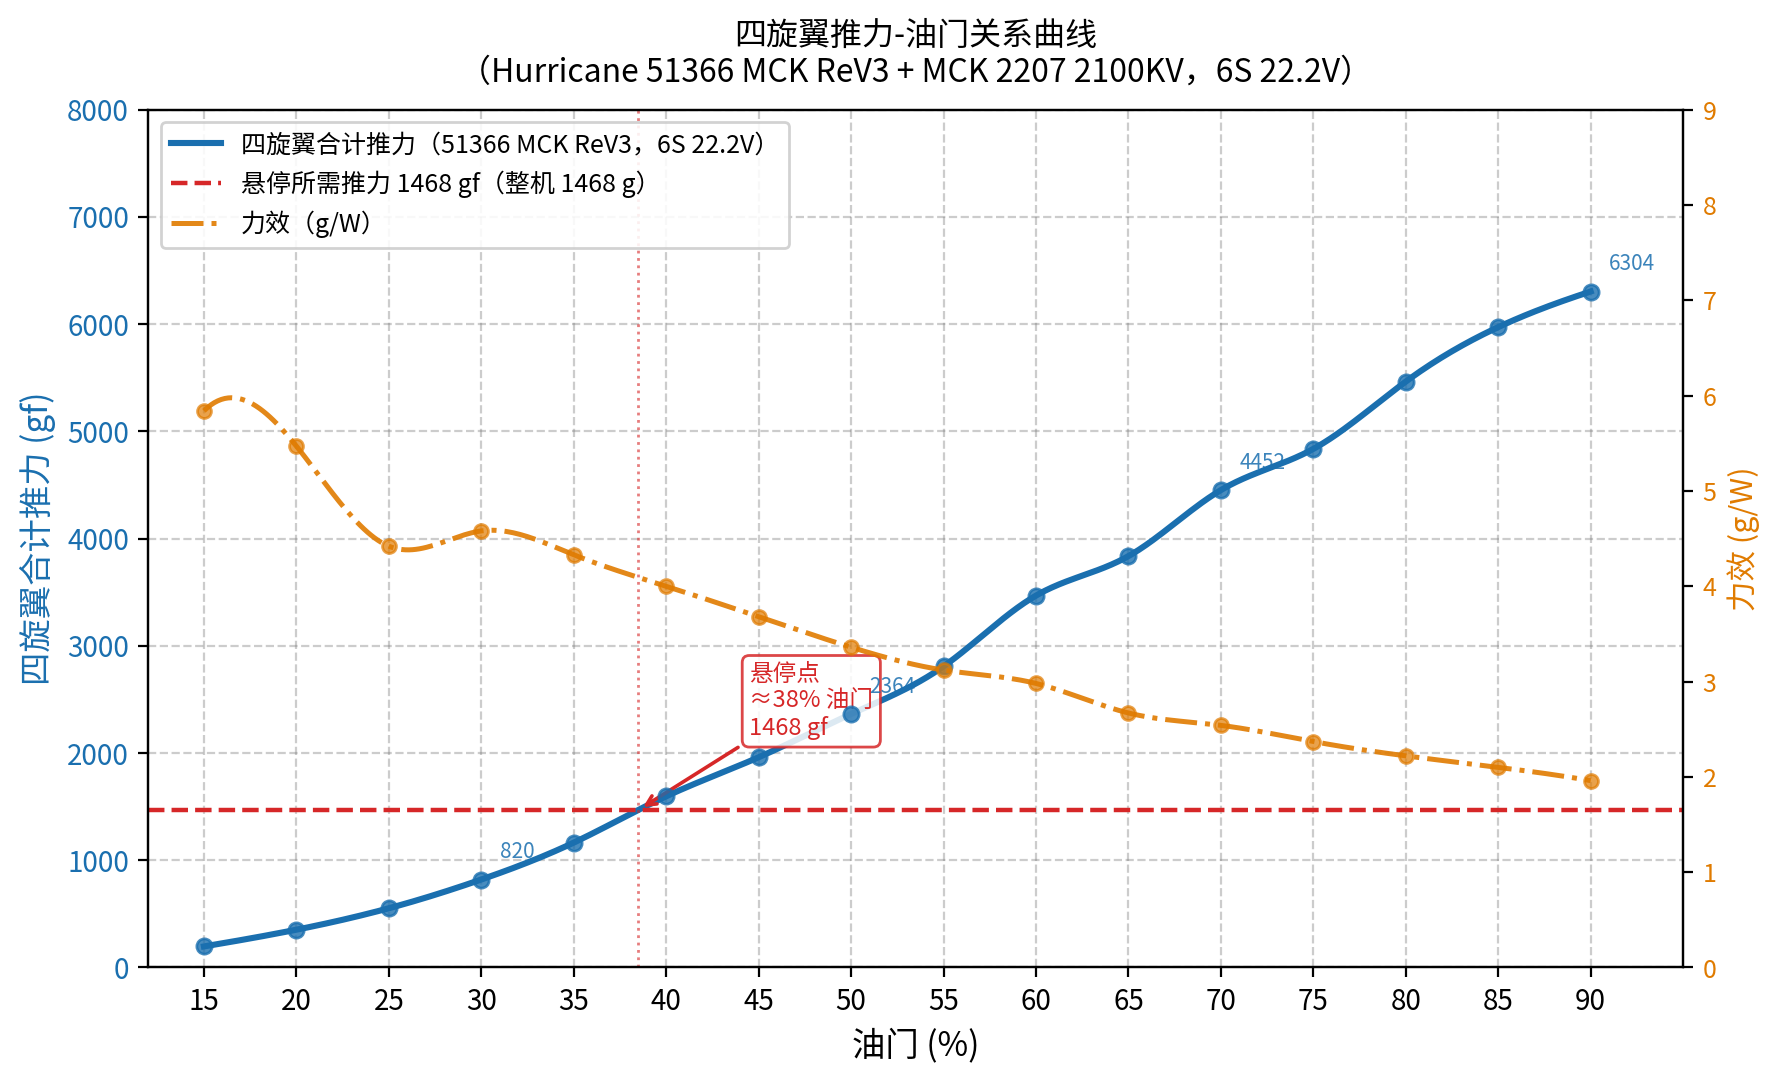
\includegraphics[width=0.85\textwidth]{figures/fig4_1_thrust_curve.png}
    \caption{四旋翼推力-油门关系曲线（6S 22.2V）}
    \label{fig:thrust_curve}
\end{figure}

由表~\ref{tab:thrust_data}及曲线图可知，系统悬停所需总推力 1468\,gf
约在 35\%$\sim$40\% 油门区间实现，\textbf{悬停工作油门约为 38\%}。
50\% 油门时推重比达 1.61，满足设计指标（$\geq 1.5$）要求，
动力储备充裕，具备良好的抗扰与机动能力。

% ----------------------------------------------------------

\section{气动阻力分析}
对于带有大面积遮蔽结构的飞行系统而言，气动载荷是影响飞行稳定性和动力消耗的关键因素。
本节将从垂直与侧向两个维度对系统的气动阻力进行分析。

\subsection{载荷位置对气动性能的影响}
多旋翼飞行器的气动性能受载荷位置影响显著。
Seth等人通过CFD仿真与实飞验证系统研究了载荷位于旋翼平面上方与下方两种配置的气动差异，
结果表明：载荷置于旋翼下方时，旋翼下洗流受到阻挡，
湍流强度显著增大，推力损失可达15\%$\sim$20\%，
俯仰/横滚姿态误差率约为20\%；
而当载荷置于旋翼上方时，下洗流路径畅通，
即使载荷覆盖面积达到桨盘面积的50\%，
推力损失可忽略不计，姿态误差率仅约0.1\%\cite{seth2023}。

本系统中，充气伞体主要结构位于旋翼平面\textbf{上方}，
与上述研究所验证的气动最优载荷位置完全一致，
从根本上避免了载荷对旋翼下洗流的干扰。
因此，以下分析更加关注侧向风载荷对系统姿态的影响。

\subsection{垂直方向气动分析}
充气伞面相对于旋翼桨盘位于上方，旋翼尾流在通过桨盘后向下加速。
伞面位于桨盘上方且面积相对于桨盘面积较大，
旋翼下洗流对伞面的直接影响可忽略不计。
在悬停工况下，伞面垂直方向气动阻力主要为静压差引起的上下面压差，
由于飞行速度接近零，此项气动力极小，对悬停推力需求的影响可忽略。

\subsection{侧向风载荷分析}
在侧风条件下，充气伞面及气柱骨架会受到侧向气动力。
根据第三章的几何设计，伞面呈拱形，具有约 12.8° 的平均倾角，其实际边长为 0.779\,m。
侧风吹袭时，系统的侧向有效迎风面积 $S_{\text{side}}$ 主要由伞面的倾斜投影决定：
\begin{equation}
    S_{\text{side}} = S_{\text{umbrella}} \times \sin(\alpha) = (0.779)^2 \times \sin(12.8^\circ) \approx 0.135\,\text{m}^2
\end{equation}
以侧风速度 $V_w = 3$\,m/s 为分析工况，采用平板阻力系数 $C_D \approx 1.3$，
系统受到的侧向气动阻力为：
\begin{equation}
    F_{\text{drag}} = \frac{1}{2}\rho V_w^2 C_D S_{\text{side}}
                    = \frac{1}{2} \times 1.225 \times 9 \times 1.3 \times 0.135
                    \approx 0.97\,\text{N} \approx 99\,\text{gf}
    \label{eq:drag}
\end{equation}
在 50\% 油门时，四旋翼合计推力约 2364\,gf。
侧向阻力（99\,gf）仅占50\%推力的约 4.2\%。
这表明伞面的 12.8° 倾角设计不仅有利于排水，还有效减小了侧向迎风面积，
使得系统具备极其充裕的侧向控制裕量，足以抵抗 3\,m/s 甚至更高级别的侧风扰动。

\section{续航时间估算}

基于式~(\ref{eq:actual_power})的悬停功率估算结果（$P \approx 217$\,W），
对两种供电形态下的续航时间进行理论估算。

\subsection{系留供电模式}

地面电源采用6S 10000\,mAh锂聚合物电池，
标称电压22.2\,V，储能约222\,Wh。
考虑电池放电效率、线缆损耗等实际因素（综合效率系数取0.65），
实际可用能量约144\,Wh，理论续航时间：

\begin{equation}
    t_{\text{tether}} = \frac{222 \times 0.65}{217} \times 60 \approx 40\,\text{min}
    \label{eq:endurance_tether}
\end{equation}

\subsection{自载电池模式}

机载电池采用6S 1500\,mAh，储能约33.3\,Wh，
理论续航时间：

\begin{equation}
    t_{\text{onboard}} = \frac{33.3 \times 0.65}{217} \times 60 \approx 6\,\text{min}
    \label{eq:endurance_onboard}
\end{equation}

自载模式主要用于功能验证与应急返航，其续航时间满足短时使用需求。
系留模式约40\,min的理论续航远超设计指标（$\geq 15$\,min），
在实际使用场景中具有充裕的使用时长。


\section{重心位置分析}

\subsection{重心高度估算}

以旋翼平面为基准面（$z = 0$），向上为正方向，
对各部件质心高度进行估算，如表~\ref{tab:cg_analysis}所示。

\begin{longtable}{lrrr}
    \caption{各部件质心高度与重心贡献}
    \label{tab:cg_analysis} \\

    % -------- 第一页表头 --------
    \toprule
    部件 & 质量 $m_i$ (g) & 质心高度 $z_i$ (mm) & $m_i z_i$ (g$\cdot$mm) \\
    \midrule
    \endfirsthead

    % -------- 续页表头 --------
    \multicolumn{4}{l}{\small 续表~\ref*{tab:cg_analysis}} \\[2pt]
    \toprule
    部件 & 质量 $m_i$ (g) & 质心高度 $z_i$ (mm) & $m_i z_i$ (g$\cdot$mm) \\
    \midrule
    \endhead

    % -------- 每页底部（非末页）--------
    \midrule
    \multicolumn{4}{r}{\small 接下页} \\
    \endfoot

    % -------- 最后一页底部 --------
    \bottomrule
    \endlastfoot

    % -------- 表格内容 --------
    电机 $\times 4$   & 320  &  0    &     0 \\[3pt]
    ESC $\times 4$    & 100  & $-$10 & $-$1000 \\[3pt]
    桨叶 $\times 4$   &  52  &  5    &   260 \\[3pt]
    Pixhawk 6C        &  38  &  40   &  1520 \\[3pt]
    GPS模块           &  30  &  50   &  1500 \\[3pt]
    接收机            &  15  &  35   &   525 \\[3pt]
    PLA节点结构件     & 600  &  5    &  3000 \\[3pt]
    气柱骨架          & 150  &  0    &     0 \\[3pt]
    TPU伞面          & 150  &  20   &  3000 \\[3pt]
    线缆与紧固件      &  13  &  0    &     0 \\
    \midrule
    \textbf{合计}     & \textbf{1468} & — & \textbf{8805} \\

\end{longtable}

整机质心高度：

\begin{equation}
    z_{\text{CG}} = \frac{\sum m_i z_i}{\sum m_i} = \frac{8805}{1468} \approx +6.0\,\text{mm}
    \label{eq:cg_height}
\end{equation}

整机质心位于旋翼平面\textbf{上方约6\,mm}处。

\subsection{重心偏高的影响分析}

质心位于旋翼平面以上，意味着系统在横向扰动下存在轻微的正反馈倾向，
即飞行器倾斜时重力分量会增大倾斜趋势。
然而，本系统质心偏高幅度仅约6\,mm，相对于1230\,mm的旋翼轴距而言极小（约0.5\%），
其对飞行稳定性的影响在正常PID控制范围内完全可以补偿，
无需进行配重调整或特殊控制策略设计。
飞控系统的PID参数整定策略将在第五章详细展开。


\section{本章小结}

本章完成了飞行雨伞系统动力系统的理论设计与选型。
整机起飞质量预算 1468\,g，对应悬停总升力需求 14.40\,N。
通过动量理论推导，悬停诱导速度约 10.56\,m/s，
理论悬停功率约 217\,W（含效率修正）。
选用 SIRIUS 2306.5-1850KV 电机配 51366 MCK v3 桨叶，
50\% 油门时推重比 2.32，悬停工作油门约 26\%$\sim$30\%。
系留模式理论续航约 40\,min，自载模式约 6\,min，均达到设计指标。
整机质心位于旋翼平面上方约 6\,mm，对飞行稳定性的影响可忽略。
上述计算结果将在第五章飞控参数整定中作为输入使用。

需要说明的是，以上质量数据为设计阶段的理论估算值；
第七章实测整机质量为 1683\,g，超出预算约 14.6\%，
具体原因见第七章 7.1.2 节分析。
